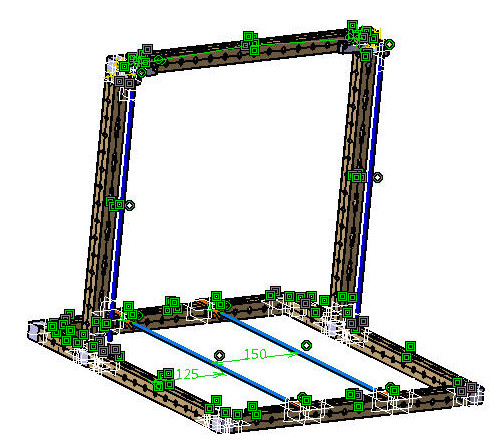
\includegraphics[width=10cm]{frame.jpg}
\section{Présentation}
\subsection{Cadre du projet}
Une imprimante 3D est une machine qui permet de reproduire des pièces %
plus ou moins complexes par apport de matière. Il existe plusieurs types %
d'imprimantes, selon le principe d'apport de matière utilisé. Le prérimètre %
de ce projet est une imprimante qui extrude du plastique à déposer couches %
par couches.
%
\subsection{Objectif}
Le principal objectif est, évidement, de construire une imprimante 3D. Cette %
imprimante fonctionnera sur le principe d'extrusion de matière plastique. Je %
m'appuie sur les imprimantes Reprap (http://reprap.org/wiki/RepRap/fr). Dans %
cette perspective, je m'autorise à réutiliser, modifier, adapter des pièces %
conçues pour d'autres imprimantes Reprap.%
%
Une contrainte forte de ce projet est le budget. En référence, une imprimante %
Reprap i3 en kit est vendue 450\euro{} sans l'électronique de commande (600\euro{} tout %
compris). Mon objectif est de limiter mon budget à 200\euro{}. C'est difficilement %
atteignable, mais pas impossible.
%
\subsection{Les imprimantes RepRap}
Le principe de ces imprimantes est qu'elles sont réplicables. Concrêtement, %
pour fabriquer une imprimante RepRap, il faut imprimer des pièces. Mon projet %
repose sur ce principe. En effet, pour des questions de facilité (je m'affranchis %
de certains usinages complexe), la plupart des supports seront imprimés.